% ============================================================
% ICTAI 2026 — Ulysses-MTRAG (DOUBLE-BLIND: anonymous)
% \documentclass[conference]{IEEEtran}; bib: references_ictai.bib
% All numbers from the full 100-conversation runs (retrieval: mtrag_eval.json;
% generation: mtrag_gen.json; judge subset: analyze_judge_subset.py).
% Submission-ready. One open slot: the anonymized repository URL (add before
% submitting). The dedicated fresh human-annotation study is deferred to future
% work (page budget); RQ2 stands on the existing expert-label audit.
% ============================================================
\documentclass[conference]{IEEEtran}
\IEEEoverridecommandlockouts
\usepackage{cite}
\usepackage{amsmath,amssymb,amsfonts}
\usepackage{graphicx}
\usepackage{booktabs}
\usepackage{multirow}
\usepackage{url}
\usepackage[T1]{fontenc}
\usepackage[utf8]{inputenc}
\usepackage[brazil,english]{babel}

\begin{document}

\title{Ulysses-MTRAG: A Synthetic Multi-Turn Benchmark for\\
Retrieval-Augmented Generation over Brazilian Legal Text}

\author{\IEEEauthorblockN{Anonymous Author(s)}
\IEEEauthorblockA{\textit{Double-blind submission} \\
\textit{Affiliation withheld for review}\\
anonymous@example.org}}

\maketitle

\begin{abstract}
Retrieval-augmented generation (RAG) for legal assistance is inherently
conversational, yet existing Brazilian-Portuguese legal information retrieval
resources are single-turn and retrieval-only. We introduce \textbf{Ulysses-MTRAG},
a synthetic multi-turn RAG benchmark for Brazilian legislative dialogue. Each
session anchors its first turn in a real expert query carrying human relevance
judgments (Ulysses-RFCorpus); an LLM then generates coherent follow-up turns, and
an LLM judge distinct from the generator assesses the relevance of retrieved
documents. Using the benchmark, we answer three questions. First, how does
retrieval quality evolve across turns, and does dialogue history help? Under four
context strategies and two retrievers, quality degrades significantly with turn
depth, and the best strategy is \emph{retriever-dependent}: dense retrieval does no
better with history than with the current turn alone, whereas lexical BM25 is
significantly best with the full dialogue history, which acts as query expansion.
Second, does model scale improve generation faithfulness? A size- and
family-controlled study (7B to 72B parameters) shows that model family dominates
parameter count: a well-chosen 8B model is more faithful than 14B and 31B models
from other families and competitive with a 72B model nine times its size, while
retrieval degradation propagates to generation only weakly (Spearman
$\rho\!\le\!0.21$). Third, how reliable is the LLM relevance judge? Against
pre-existing expert labels, full-pool agreement is modest ($0.58$)---dominated by
pooled documents the experts never assessed---but rises to $0.94$ on the subset
they explicitly labeled. We will release the benchmark, prompts, and code; an
anonymized repository accompanies this submission.
\end{abstract}

\begin{IEEEkeywords}
retrieval-augmented generation, multi-turn dialogue, legal NLP, information
retrieval, LLM-as-a-judge, Brazilian Portuguese
\end{IEEEkeywords}

% ============================================================
\section{Introduction}
Legal information seeking is conversational: an analyst refines an initial
question across several turns. Retrieval-augmented generation (RAG)
\cite{Lewis2020RAG} is the dominant paradigm for grounding such assistance, but
Brazilian-Portuguese legal IR resources---Ulysses-RFCorpus \cite{Vitorio2024},
JurisTCU \cite{Fernandes2026JurisTCU}, and the JU\'A benchmark
\cite{Pereira2026JUA}---are \emph{single-turn} and stop at retrieval. Multi-turn
legal RAG in Portuguese has, to our knowledge, not yet been studied.

We address this gap with \textbf{Ulysses-MTRAG}, a synthetic multi-turn benchmark
for Brazilian legislative dialogue. Rather than transplanting an existing recipe,
our construction targets both scalability and ecological validity: each session is
anchored in a \emph{real} expert query that carries human relevance judgments, and
only the follow-up turns are LLM-generated. This human-anchored design sets
Ulysses-MTRAG apart from prior multi-turn benchmarks. MTRAG \cite{Katsis2025MTRAG}
is fully human-authored---accurate, but unscalable. CORAL \cite{Cheng2025CORAL}
derives conversations automatically from Wikipedia---scalable, but without expert
relevance ground truth. Anchoring in pre-existing expert judgments lets us do
something neither prior design supports: audit the LLM relevance judge against
experts \emph{inside} the benchmark itself. Our contributions are:
\begin{itemize}
  \item \textbf{Ulysses-MTRAG}: a multi-turn legal RAG benchmark of 100 four-turn
  sessions over 105{,}669 legislative bills, with human-anchored first turns,
  LLM-generated follow-ups, and pooled relevance labels from a judge distinct from
  the generator.
  \item A \textbf{multi-turn retrieval analysis} across four context strategies and
  two retrievers, with paired significance tests, showing per-turn degradation and a
  strategy--retriever interaction: the optimal use of dialogue history reverses
  between dense and lexical retrieval.
  \item A \textbf{size- and family-controlled generation study} (7B--72B) showing
  that faithfulness is governed more by model family than by parameter count: the
  best 8B model outperforms 14B and 31B models from other families and is
  statistically indistinguishable from a 72B model nine times its size. Scaling up
  is thus not a reliable route to faithful legal RAG in this domain.
  \item Evidence that \textbf{retrieval degradation propagates to generation only
  weakly}: faithfulness declines far less steeply than retrieval quality across
  turns, and correlates weakly with it at the turn level.
  \item A \textbf{reliability assessment} of the LLM relevance judge against
  pre-existing expert labels, disentangling the pooling-incompleteness confound: on
  the subset of documents the experts explicitly labeled, raw agreement is $0.94$.
\end{itemize}

\noindent\textbf{Research questions.}
\textbf{RQ1}: How does retrieval quality evolve across turns, and do history-aware
context strategies outperform using the current query alone?
\textbf{RQ2}: How reliable is the LLM relevance judge against expert labels?
\textbf{RQ3}: Does model scale improve dialogue-grounded generation, and does
retrieval degradation propagate to the generated answers?

% ============================================================
\section{Related Work}
\textbf{RAG evaluation and LLM-as-a-judge.} LLM judges are now standard for
evaluating generation \cite{Zheng2023MTBench,Liu2023GEval,Kim2024Prometheus2} and
RAG specifically \cite{Es2024RAGAS}, including relevance assessment
\cite{Thomas2024Searcher,Upadhyay2024UMBRELA,Faggioli2023Perspectives}. They carry
known biases---position \cite{Wang2024Unfair}, verbosity \cite{Zheng2023MTBench},
and self-preference \cite{Panickssery2024SelfPref}---which motivates our use of a
judge distinct from the generator. Relevance labels are also highly prompt-sensitive
\cite{Arabzadeh2025Prompt}; rather than blunt strictness we adopt a rubric with
reason-then-label prompting \cite{Liu2023GEval} and quantify agreement with expert
labels, reporting agreement statistics
\cite{Calderon2025AltTest,Hashemi2024LLMRubric}.

\textbf{Multi-turn / conversational RAG.} Conversational QA and RAG benchmarks
\cite{Katsis2025MTRAG,Cheng2025CORAL,Qu2020ORConvQA} and conversational query
rewriting \cite{Anantha2021QReCC,Elgohary2019CANARD,Mao2023LLM4CS} establish the
context strategies we compare. Whether history helps is mixed: ORConvQA
\cite{Qu2020ORConvQA} finds history beneficial on human data, while synthetic
pipelines tend to produce self-contained questions \cite{Vlachos2025Synthetic}---%
decontextualized in the sense of \cite{Choi2021Decontextualization}---a tendency
our benchmark lets us quantify and stress-test. Degradation over long dialogues is also
documented \cite{Laban2025Lost}. Relative to MTRAG and CORAL, Ulysses-MTRAG differs
on three axes: turn provenance (human seed + synthetic follow-ups, vs.\ fully human
in MTRAG and fully automatic in CORAL), relevance-label provenance (expert judgments
at the seed turn, enabling in-benchmark judge auditing), and domain (legislative
bills in Portuguese, including a low-resource language setting neither covers).

\textbf{Long-document retrieval and chunking.} Passage-level indexing of long
documents is the canonical mitigation when inputs exceed model limits
\cite{Dai2019Deeper,Karpukhin2020DPR}, though the optimal retrieval-unit
granularity remains debated \cite{Jiang2024LongRAG}. Embedding models have hard
token limits (BGE-M3: 8192 tokens \cite{Chen2024BGEM3}) and degrade on long inputs
\cite{Zhou2024LengthCollapse}; BM25 remains a strong baseline,
especially in lexically rich domains \cite{Robertson2009BM25,Thakur2021BEIR}.

\textbf{Legal IR in Portuguese and synthetic data.} We build on Brazilian legal
IR resources \cite{Vitorio2024,Fernandes2026JurisTCU,Pereira2026JUA,Junior2025BRTaxQA,LuzdeAraujo2018LeNERBr}.
Synthetic data generation with LLMs is well established for IR
\cite{Bonifacio2022InPars,Dai2023Promptagator} and as an evaluation proxy
\cite{Chiang2023Can}; anchoring synthetic data in human ground truth mitigates the
risks of fully recursive generation \cite{Shumailov2024Collapse}.

% ============================================================
\section{Retrieval Setup}
\label{sec:foundation}
Our experiments use two standard retrievers: lexical BM25 \cite{Robertson2009BM25}
and dense BGE-M3 \cite{Chen2024BGEM3}. The benchmark corpus is legislative bills,
whose official summaries (\emph{ementas}) are short and fit comfortably within
the encoder's window. The multi-turn experiments therefore index each bill by its
full summary, with no chunking needed.

\textbf{A length boundary, and why our benchmark avoids it.} Before the multi-turn
analysis, we check whether this retrieval stack has a length limitation on
Brazilian legal text, using the regulatory sub-domain of JU\'A
\cite{Pereira2026JUA} (NormasTCU; $\sim$12k-token norms, $n{=}46$ queries) as a
stress test. It does: whole-document dense retrieval \emph{collapses} there---no
relevant norm appears in any top-10, yielding nDCG@10$=$0.000 across all
queries---while lexical BM25 attains 0.328 (Table~\ref{tab:chunking}). The
mechanism is length: each norm far exceeds BGE-M3's 8192-token window, so the
single vector indexed per document is computed from a truncated prefix that omits
the query-relevant passages \cite{Chen2024BGEM3,Zhou2024LengthCollapse}. The
standard passage-level remedy---splitting each norm into sub-8k chunks, indexing
the chunks, and mapping retrieved chunks back to documents
\cite{Dai2019Deeper,Karpukhin2020DPR}---recovers dense retrieval to parity with
BM25 (nDCG@10$=$0.330; BM25 still retains better recall). This confirms the
boundary is real and gives us a tested mitigation, but our own bill corpus never
approaches it: bill summaries are far short of 8k tokens, so the multi-turn
benchmark below indexes them whole, with no chunking required.

\begin{table}[t]
\caption{Retrieval on NormasTCU ($n{=}46$). Whole-document dense retrieval
collapses on $\sim$12k-token norms; chunk-level indexing recovers parity with BM25.}
\label{tab:chunking}
\centering
\begin{tabular}{lcccc}
\toprule
\textbf{Method} & \textbf{nDCG@5} & \textbf{nDCG@10} & \textbf{R@10} & \textbf{MRR} \\
\midrule
BM25 (full text)      & 0.287 & \textbf{0.328} & 0.339 & 0.454 \\
Dense, whole document & 0.000 & 0.000 & 0.000 & 0.000 \\
Dense, chunk-level    & 0.317 & \textbf{0.330} & 0.294 & 0.559 \\
\bottomrule
\end{tabular}
\end{table}

% ============================================================
\section{The Ulysses-MTRAG Benchmark}
\label{sec:benchmark}
\textbf{Construction.} Session construction has three steps: seed selection, turn
generation, and quality control.

\emph{Seed selection.} We start from the 692 queries of the public Ulysses-RFCorpus
release, each carrying graded relevance judgments (relevant / partially relevant /
irrelevant) produced by the legislative consultants of the Brazilian Chamber of
Deputies \cite{Vitorio2024}, over a corpus of 105{,}669
bills.\footnote{Counts refer to the public release we use (692 queries;
105{,}669 bills); the dataset paper reports 693 queries and 105{,}681 documents
\cite{Vitorio2024}.} We keep only queries with at least three (partially) relevant
bills, embed the remaining query texts with BGE-M3, and cluster them with
$k$-means ($k{=}100$, fixed seed). One representative query per cluster becomes a
session seed, giving a diverse, non-redundant set of 100 seeds; each seed becomes
Turn~1 and inherits its expert relevance labels.

\emph{Turn generation.} Turns~2--4 are generated by an instruction-tuned LLM
(Qwen2.5-72B), conditioned on the full session history and prompted to produce a
coherent next question of a \emph{prescribed} type---follow-up, clarification,
non-standalone, comparative, or temporal. We designed this five-type scheme around
the conversational challenges MTRAG emphasizes: non-standalone and comparative
questions, and answerability \cite{Katsis2025MTRAG}.

\emph{Quality control.} The generator is instructed to stay on-topic and not
repeat earlier turns. We discard degenerate generations---empty, duplicated, or
off-topic---and regenerate them. The result is 100 four-turn sessions (400 turns
total); Fig.~\ref{fig:example} shows one. A Portuguese-specialized generator
(e.g., Gaia/Sabi\'a) is left for future work.

\begin{table}[t]
\caption{Ulysses-MTRAG composition: realized turn-type and answer-type
distributions over the 300 generated turns (T2--T4). Turn types are prescribed by
sampling at generation time; answer types are as labeled by the generator.}
\label{tab:stats}
\centering
\begin{tabular}{lr@{\hspace{1.2em}}lr}
\toprule
\textbf{Turn type} & \textbf{\%} & \textbf{Answer type} & \textbf{\%} \\
\midrule
follow-up      & 47.0 & answerable   & 99.3 \\
clarification  & 20.3 & partial      &  0.7 \\
non-standalone & 11.3 & unanswerable &  0.0 \\
comparative    & 11.0 &              &      \\
temporal       & 10.3 &              &      \\
\bottomrule
\end{tabular}
\end{table}

Table~\ref{tab:stats} reports the realized composition. Because the type
distribution is a construction input (sampled by design), we do not read it as a
finding; what \emph{is} informative is that only $11.3\%$ of generated turns are
explicitly non-standalone, so the benchmark---like other synthetic
conversational-QA pipelines \cite{Vlachos2025Synthetic}---consists largely of
self-contained (decontextualized \cite{Choi2021Decontextualization}) questions on
a shared topic. We treat this as a measurable property of the synthetic
construction recipe and stress-test its
consequences in \S\ref{sec:results} (RQ1), including a turn-type-stratified
analysis. Almost all turns are answerable ($99.3\%$); the near-absence of
unanswerable turns is a limitation we discuss in \S\ref{sec:discussion}.

\textbf{Relevance labels.} For every turn, the documents retrieved by all context
strategies are pooled and labeled once by an LLM judge (Llama-3.3-70B),
\emph{distinct from the generator} to avoid self-preference bias
\cite{Panickssery2024SelfPref}, using a graded rubric with reason-then-label
prompting \cite{Liu2023GEval}. \emph{All} retrieval scores in this paper, including
Turn~1, use these judge labels, so cross-turn comparisons rest on a single label
source; the expert labels of Turn~1 are reserved for auditing the judge itself
(\S\ref{sec:results}, RQ2). Graded labels are binarized at $0.5$ (partially
relevant counts as relevant) wherever binary agreement is computed.

\begin{figure}[t]
\small\setlength{\parindent}{0pt}
\textbf{T1} \emph{(seed, human-labeled)}: ``Criação de fundo para prevenção de desastres naturais e e recuperação de seus efeitos, para\ldots''\\
$\rightarrow$ top: \textbf{PL 295/2007} --- \emph{relevant}\\[3pt]
\textbf{T2} \emph{(follow-up)}: ``Quais são os principais critérios e mecanismos de distribuição dos recursos do fundo para\ldots''\\
$\rightarrow$ top: \textbf{PL 5067/2016} --- \emph{relevant}\\[3pt]
\textbf{T3} \emph{(clarification)}: ``Em quais situações específicas os recursos do fundo para prevenção de desastres naturais e\ldots''\\
$\rightarrow$ top: \textbf{PL 10898/2018} --- \emph{relevant}\\[3pt]
\textbf{T4} \emph{(clarification)}: ``Como são definidas as prioridades para a alocação de recursos do fundo em situações de\ldots''\\
$\rightarrow$ top: \textbf{PL 4450/2020} --- \emph{partially relevant}
\caption{A worked example from Ulysses-MTRAG: a four-turn session seeded by a real
Ulysses-RFCorpus query (T1, which additionally carries expert relevance labels)
with LLM-generated follow-ups (T2--T4). For each turn we show the top retrieved
bill and its LLM-judge relevance label. Queries are reproduced verbatim in the
original Portuguese, including typos present in the source corpus. The retrieved
bill \emph{shifts} across turns and degrades to only \emph{partially relevant} by
T4.}
\label{fig:example}
\end{figure}

% ============================================================
\section{Multi-Turn Evaluation Setup}
\label{sec:setup}
\textbf{Retrieval.} For each turn we retrieve top-$k$ ($k{=}10$) bills under four
context strategies: \emph{last-turn} (current query only), \emph{concat} (prior
queries prepended), \emph{full-history} (all prior turns), and \emph{rewrite} (a
Llama-3.1-8B model rewrites the query to standalone form)
\cite{Mao2023LLM4CS,Elgohary2019CANARD}. Per turn and per retriever, we pool the
documents retrieved by the four strategies and judge the pool once (standard
pooling), scoring each strategy with nDCG@10 on the shared labels. A persistent
judgment cache assigns identical labels to any (query, document) pair that appears
in both retrievers' pools. We run the full strategy comparison under \emph{both}
retrievers---dense BGE-M3 and lexical BM25 (\S\ref{sec:foundation})---to test
whether conclusions about dialogue history are retriever-specific.

\textbf{Generation.} To test whether retrieval degradation propagates to answers,
each turn's top-5 last-turn-retrieved bills are passed, with a history-aware
prompt, to five open-weight instruction-tuned small language models (SLMs). We
chose these five to span the size range at competitive quality: Qwen2.5-7B
\cite{Qwen2024Qwen25}, Qwen3-8B \cite{Yang2025Qwen3}, Ministral-8B, Phi-4 (14B)
\cite{Abdin2024Phi4}, and Gemma-4-31B. This spread lets the effect of scale be
read directly from the comparison. We score each answer on three axes adapted
from MTRAG's generation evaluation \cite{Katsis2025MTRAG}: (i) \emph{context
faithfulness} (reference-less, RAGAS-style \cite{Es2024RAGAS}), judged by
Llama-3.3-70B \cite{Grattafiori2024Llama3}; (ii) \emph{reference similarity} to
an oracle answer via BERTScore-F1
\cite{Zhang2020BERTScore} and ROUGE-L \cite{Lin2004ROUGE}; and (iii) an LLM-judge
comparison against the oracle answer. The oracle (Qwen2.5-72B) receives the
\emph{same} retrieved context and history as the evaluated models. Two design
facts must be stated openly: the oracle is the same model that generated the
follow-up questions, and it shares a family with two evaluated models. The judge
is distinct from both the generators and the oracle, and our headline claims rest
on the reference-less faithfulness axis, which does not use the oracle at all;
empirically, the reference-based metrics do not favor the oracle's family either
(Phi-4 leads both, \S\ref{sec:results}).

\textbf{Implementation.} Generation uses temperature $0.1$ (max 1024 tokens);
judging uses temperature $0$. Dense retrieval uses BGE-M3 embeddings with FAISS
\cite{Douze2024Faiss}; BM25 is BM25Okapi ($k_1{=}1.5$, $b{=}0.75$); NormasTCU
chunking uses 3{,}000-character chunks with 400-character overlap; seed clustering
uses $k$-means with a fixed random seed. BERTScore uses multilingual BERT. Models
are accessed through OpenAI-compatible APIs. All prompts (turn generation, query
rewriting, relevance rubric, faithfulness judging), model identifiers, and
configuration files are included in the anonymized repository accompanying this
submission.

% ============================================================
\section{Results}
\label{sec:results}
\textbf{RQ1 --- per-turn degradation and the strategy--retriever interaction.}
Table~\ref{tab:mtrag} reports nDCG@10 by retriever, strategy, and turn; strategies
coincide at T1, where no history exists. Under both retrievers retrieval quality
\emph{declines significantly as the conversation deepens}: for dense last-turn,
nDCG@10 falls from $0.876$ (seed) to $0.617$ at T3 ($\Delta{=}0.26$, paired Wilcoxon
$p<10^{-12}$; Fig.~\ref{fig:retrieval}). The largest single drop (T1$\to$T2)
coincides with the switch from human-authored seed queries to synthetic follow-ups,
so we read depth-degradation primarily from the continued decline within the
synthetic turns.

\emph{Which context strategy is best depends on the retriever.} For dense BGE-M3, no
history-aware strategy beats last-turn (means within $\approx$0.02; last-turn is
indistinguishable from concat and full-history, Holm $p\ge0.17$, and better than
rewrite, $p_{\text{adj}}{=}0.023$): concatenating history dilutes the single query
embedding. For lexical BM25 the ranking \emph{reverses}---full-history is best and
last-turn the \emph{worst} strategy ($0.741$ vs.\ $0.668$ all-turn mean; a $+0.097$
gap over T2--T4, paired Wilcoxon $p<10^{-7}$)---because appending prior turns acts as
query expansion, supplying lexically matching legal terms. Using only the current
turn is thus a safe default for dense retrieval, but a poor one for lexical
retrieval, where the opposite holds. This interaction cautions against drawing
conclusions about conversational context from a single retriever.

Stratifying the dense results by turn type localizes the last-turn null result:
explicitly non-standalone turns are the hardest (last-turn nDCG@10 $0.52$ vs.\
$0.64$--$0.73$ for the other types) and history-aware dense strategies do not
recover them (concat $0.40$, full-history $0.43$, rewrite $0.40$), while
full-history helps only modestly on clarification ($0.69$ vs.\ $0.66$) and temporal
($0.68$ vs.\ $0.64$) turns---consistent with the self-contained questions synthetic
pipelines are known to produce \cite{Vlachos2025Synthetic}, decontextualized in the
sense of \cite{Choi2021Decontextualization}; contrast ORConvQA
\cite{Qu2020ORConvQA}, where history helps on human dialogue. One caveat: pooled
documents are judged against the turn text itself, which may favor last-turn on
non-standalone turns; history-aware judging is future work.

\begin{table}[t]
\caption{Multi-turn retrieval (nDCG@10) by retriever, context strategy, and turn
position (100 conversations; per retriever, a single LLM-judged pool per turn scores
all strategies, including T1, so strategies coincide at T1). Best strategy per
retriever (all-turn mean) in bold. The ordering \emph{reverses} between dense and lexical retrieval.}
\label{tab:mtrag}
\centering\small\setlength{\tabcolsep}{4pt}
\begin{tabular}{llccccc}
\toprule
\textbf{Retr.} & \textbf{Strategy} & \textbf{T1} & \textbf{T2} & \textbf{T3} & \textbf{T4} & \textbf{mean} \\
\midrule
\multirow{4}{*}{\rotatebox[origin=c]{90}{BGE-M3}}
 & last-turn    & 0.876 & 0.727 & 0.617 & 0.636 & \textbf{0.714} \\
 & rewrite      & 0.876 & 0.718 & 0.587 & 0.604 & 0.696 \\
 & concat       & 0.876 & 0.718 & 0.621 & 0.557 & 0.693 \\
 & full-history & 0.876 & 0.695 & 0.605 & 0.597 & 0.693 \\
\midrule
\multirow{4}{*}{\rotatebox[origin=c]{90}{BM25}}
 & full-history & 0.900 & 0.755 & 0.670 & 0.637 & \textbf{0.741} \\
 & concat       & 0.900 & 0.731 & 0.624 & 0.449 & 0.676 \\
 & rewrite      & 0.900 & 0.652 & 0.587 & 0.564 & 0.676 \\
 & last-turn    & 0.900 & 0.641 & 0.580 & 0.551 & 0.668 \\
\bottomrule
\end{tabular}
\end{table}

\begin{figure}[t]
\centering
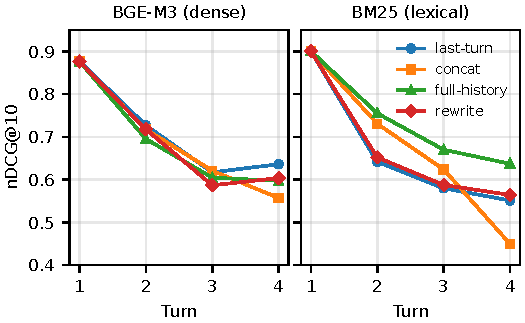
\includegraphics[width=\columnwidth]{fig_retrieval_turns.pdf}
\caption{Retrieval nDCG@10 by turn for the four context strategies, under dense
(left) and lexical (right) retrieval (100 conversations). Quality drops after the
seed turn under both, but the best strategy \emph{reverses}: last-turn leads for
dense embeddings, full-history leads for BM25.}
\label{fig:retrieval}
\end{figure}

\textbf{RQ2 --- judge reliability against expert labels.}
We audit the LLM judge against the pre-existing expert labels on the dense-run
Turn-1 pool, reporting raw agreement alongside Cohen's~$\kappa$ \cite{Cohen1960}
and the Prevalence- and Bias-Adjusted Kappa (PABAK) \cite{Byrt1993PABAK}, which
corrects $\kappa$ for skewed class prevalence. Over the full pool ($n{=}1000$
query--document pairs), agreement is modest (raw $0.58$, $\kappa{=}0.27$): the judge labels $69\%$ of
pooled documents relevant while the sparse expert labels cover far fewer ($29\%$),
exactly the pattern expected when a retriever surfaces topically relevant documents
the original annotators never assessed and the pooling convention counts them as
irrelevant \cite{Voorhees2000}. The confound is testable: restricting the
comparison to the $n{=}305$ pool documents the experts \emph{explicitly} labeled
(including explicit ``irrelevant''), raw agreement rises to $\mathbf{0.938}$
(PABAK $0.875$). On this subset $\kappa$ remains modest ($0.39$) because
$95\%$ of explicitly labeled documents are relevant---the classic kappa paradox of
high agreement under skewed prevalence \cite{Feinstein1990,Byrt1993PABAK}. Taken
together, the two views indicate the judge tracks expert judgments closely where
expert opinion is known, and the full-pool disagreement is dominated by label
incompleteness rather than judge error; relevance judgment also varies among human
assessors themselves \cite{Voorhees2000}. A dedicated human annotation over the
full retrieved pool remains desirable future work (\S\ref{sec:discussion}).

\textbf{RQ3 --- does scale help generation, and does degradation propagate?}
Table~\ref{tab:gen} reports generation quality by model with parameter counts.
\emph{Model family dominates parameter count.} The most faithful open model is
Qwen3-8B ($0.808$, 95\% CI $[0.778, 0.837]$), which significantly outperforms the
14B Phi-4 ($0.762$) and the 31B Gemma-4 ($0.725$; paired $\Delta{=}0.083$, Wilcoxon
$p<10^{-5}$): scaling to a larger model of a \emph{different} family does not help
here. Scale does help \emph{within} a family, but with steep diminishing returns:
across the Qwen models faithfulness rises $0.781$ (7B) $\to 0.808$ (8B) $\to 0.841$
(72B, the oracle), yet only the full $10\times$ span is significant (7B$\to$72B,
$p{=}0.001$); the $9\times$ step from 8B to 72B is not ($+0.033$, $p{=}0.074$), and
the 72B additionally answers questions it authored, an advantage that inflates its
score. Practically, a well-chosen 8B model is thus competitive with a 72B model nine
times its size; parameter count alone predicts faithfulness far less reliably
than model family and training do.
Faithfulness and reference similarity also decouple: Qwen3-8B is most faithful, yet
Phi-4 is closest to the oracle answer (BERTScore $0.830$, ROUGE-L $0.472$), and since
Phi-4 is not from the oracle's family, family bias does not dominate the
reference-based metrics. The third planned axis, an LLM-judge comparison against the
oracle answer, did not discriminate among models (all $\approx0.50$); we report this
as a negative finding---single-scale equivalence rating of two free-form legal
answers is too coarse---and exclude it from Table~\ref{tab:gen}.

Retrieval degradation \emph{propagates to generation, but weakly}. Mean
faithfulness falls from $0.802$ (T1) to $0.751$ (T4) and ROUGE-L from $0.434$ to
$0.358$; the decline is significant for the two most faithful models (Qwen3-8B
$-0.113$, $p{=}0.006$; Qwen2.5-7B $-0.101$, $p{=}0.008$) and flat for the rest
($p>0.27$), so the leaders converge toward the pack as the dialogue deepens
(Fig.~\ref{fig:generation}). Directly correlating per-turn retrieval nDCG@10 with
generation metrics over all 2000 (turn, model) units yields weak positive
associations (Spearman $\rho{=}0.16$ for faithfulness, $0.21$ for ROUGE-L):
grounding is largely preserved even when retrieval degrades. We note the
interpretive limit of this metric: faithfulness rewards grounding in
\emph{whatever} context was retrieved, so it measures hallucination control, not
answer utility---an answer faithful to irrelevant bills scores high. Reference
similarity partially covers this gap, but since the oracle answers from the same
degraded context, cross-turn declines in ROUGE-L partly reflect reference drift.
Finally, repeating the faithfulness judging run shifts absolute scores by up to
$\approx0.05$ while preserving the model ranking; we therefore read all judge
scores comparatively.

\begin{table}[t]
\caption{Multi-turn generation quality (100 conversations, 400 turns per model):
reference-less context faithfulness and reference similarity to the oracle answer
(BERTScore-F1, ROUGE-L). Best per column (excluding the oracle) in bold; 95\%
bootstrap CIs on faithfulness are within $\pm0.03$. $^{\dagger}$Oracle model
(authored the follow-ups and serves as the similarity reference), shown as a
same-family scale anchor---faithfulness only.}
\label{tab:gen}
\centering\small\setlength{\tabcolsep}{5pt}
\begin{tabular}{lcccc}
\toprule
\textbf{Model} & \textbf{Params} & \textbf{Faithf.} & \textbf{BERTScore} & \textbf{ROUGE-L} \\
\midrule
Qwen3-8B      & 8B  & \textbf{0.808} & 0.800 & 0.398 \\
Qwen2.5-7B    & 7B  & 0.781 & 0.786 & 0.398 \\
Phi-4         & 14B & 0.762 & \textbf{0.830} & \textbf{0.472} \\
Ministral-8B  & 8B  & 0.752 & 0.762 & 0.271 \\
Gemma-4-31B   & 31B & 0.725 & 0.796 & 0.372 \\
\midrule
Qwen2.5-72B$^{\dagger}$ & 72B & 0.841 & --- & --- \\
\bottomrule
\end{tabular}
\end{table}

\begin{figure}[t]
\centering
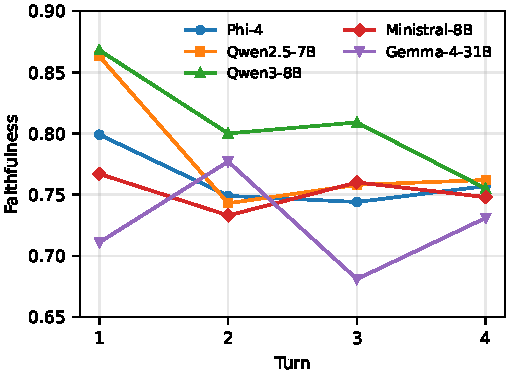
\includegraphics[width=\columnwidth]{fig_generation_turns.pdf}
\caption{Generation faithfulness by turn for the five small language models (100
conversations). The most faithful models decline significantly and converge toward
the pack, while retrieval drops far more steeply (Fig.~\ref{fig:retrieval}).}
\label{fig:generation}
\end{figure}

% ============================================================
\section{Discussion and Limitations}
\label{sec:discussion}
\textbf{What the benchmark measures.} Ulysses-MTRAG quantifies a property of
synthetic multi-turn benchmark construction: follow-ups are largely self-contained
($11.3\%$ non-standalone by design), so history-aware retrieval cannot show its
value---our stratified analysis confirms history helps only on clarification and
temporal turns. We present this as a diagnostic finding about synthetic multi-turn
pipelines in a low-resource legal domain. Benchmarks intending to stress
conversational context should enforce a higher non-standalone quota at generation
time; we leave three extensions to future work: (a) such a higher-quota
generation scheme, (b) eliciting unanswerable turns ($99.3\%$ of ours are
answerable), which MTRAG \cite{Katsis2025MTRAG} uses to test abstention, and
(c) a dedicated human annotation of the full retrieved pool to tighten the
judge-reliability bound of RQ2.

\textbf{Validity threats.}
\begin{itemize}
  \item[(i)] We evaluate two retrievers (dense and lexical) and find the strategy
  ranking reverses between them; hybrid retrieval and other dense encoders may
  behave differently again, so the specific rankings should not be
  over-generalized beyond the two families tested.
  \item[(ii)] The follow-up generator, the oracle, and two evaluated models are
  related (same model or family). We mitigate this by resting headline claims on
  the reference-less faithfulness axis, judged by a model from a different
  family, and by noting that a non-family model leads the reference-based
  metrics.
  \item[(iii)] The cross-family comparison has one model per size point, so
  family and size are partly confounded. We add a within-family Qwen ladder
  (7B/8B/72B) to isolate scale, but the 72B anchor is also the question author,
  an advantage we cannot fully remove.
  \item[(iv)] Judge-based scores vary across judging runs ($\approx0.05$ in
  absolute value, though the ranking is stable) and are LLM-judged over a
  retrieval pool; absolute values should therefore be read as comparative
  rankings, with reliability bounded in RQ2.
  \item[(v)] The benchmark covers one legislative corpus, four-turn sessions, and
  synthetic follow-ups; human-authored legal dialogue may behave differently
  \cite{Qu2020ORConvQA}.
\end{itemize}

% ============================================================
\section{Conclusion}
We presented Ulysses-MTRAG, a human-anchored synthetic multi-turn RAG benchmark
for Brazilian legislative dialogue. Retrieval degrades significantly with dialogue
depth, and the best way to use dialogue history turned out to be
retriever-dependent: inert for dense retrieval, but a significant gain for lexical
BM25. Generation faithfulness is governed more by model family than by scale---a
well-chosen 8B model is competitive with a 72B model nine times larger---and
retrieval degradation propagates to generated answers only weakly. Finally, the
LLM relevance judge agrees with expert labels on $94\%$ of the documents experts
explicitly assessed, with full-pool disagreement dominated by label incompleteness
rather than judge error. The benchmark, prompts, and code will be released; an
anonymized repository accompanies the review.

\bibliographystyle{IEEEtran}
\bibliography{references_ictai}

\end{document}
